%#! platex  -halt-on-error -file-line-error -src-specials main.tex
% Time-stamp: <2016-12-14 20:07:36 takago>

\chapter{ウェーブレット変換}
あわれといふも,なかなか疎かなり.されば,人間の儚き事は,老少不定のさかいなれば,誰の人も早く後生の一大事を心にかけて,阿弥陀仏を深く頼み参らせて,念仏申すべきものなり. あなかしこ,あなかしこ.○○○○ ○○○○○○○○○○○○○○○○○○○○○○○○○○○○○○○○○○○○○○○○○○○○○○○○○○○○○○○○○○ ○○○○○○○○○○○○○○○○○○○○○○○○○○○○○○○○○○○○○○○○○○○○○○○○○○○○○○○○ ○○○○○○○○○○○○○○○○○○○○○○○○○○○○○○○○○○○○○○○○○○○○○○○○○○○○○○ ○○○

\section{ウェーブレット}\label{AAAB}
○○○○ ○○○○○○○○○○○○○○○○○○○○○○○○○○○○○○○○○○○○○○○○○○○○○○○○○○○○○○○○○○ ○○○○○○○○○○○○○○○○○○○○○○○○○○

○○○○○○○○○○○○○○○○○○○○○○○○○○○○○○ ○○○○○○○○○○○○○○○○○○○○○○○○○○○○○○○○○○○○○○○○○○○○○○○○○○○○○○ ○○○○○○○ ○○○○○○○○○○○○○○○○○○○○○○○○○○○○○○○○○○○○○○○○○○○○○○○○○○○○○○○○○○ ○○○○○○○○○○○○○○○○○○○○○○○○○○○○○○○○○○○○○○○○○○○○○○○○○○○○○○○○ ○○○○○○○○○○○○○○○○○○○○○○○○○○○○○○○○○○○○○○○○○○○○○○○○○○○○○○ ○○○
\section{連続ウェーブレット変換}

第\ref{AAAB}節をみてね.

\subsection{桃太郎伝説}
○○○○ ○○○○○○○○○○○○○○○○○○○○○○○○○○○○○○○○○○○○○○○○○○○○○○○○○○○○○○○○○○ ○○○○○○○○○○○○○○○○○○○○○○○○○○○○○○○○○○○○○○○○○○○○○○○○○○○○○○○○ ○○○○○○○○○○○○○○○○○○○○○○○○○○○○○○○○○○○○○○○○○○○○○○○○○○○○○○ ○○○○○○○ ○○○○○○○○○○○○○○○○○○○○○○○○○○○○○○○○○○○○○○○○○○○○○○○○○○○○○○○○○○ ○○○○○○○○○○○○○○○○○○○○○○○○○○○○○○○○○○○○○○○○○○○○○○○○○○○○○○○○ ○○○○○○○○○○○○○○○○○○○○○○○○○○○○○○○○○○○○○○○○○○○○○○○○○○○○○○ ○○○

\begin{itemize}
\item やまにのぼる
\item せんたくにいく
\item ねる
\end{itemize}

○○○○ ○○○○○○○○○○○○○○○○○○○○○○○○○○○○○○○○○○○○○○○○○○○○○○○○○○○○○○○○○○ ○○○○○○○○○○○○○○○○○○○○○○○○○○○○○○○○○○○○○○○○○○○○○○○○○○○○○○○○ ○○○○○○○○○○○○○○○○○○○○○○○○○○○○○○○○○○○○○○○○○○○○○○○○○○○○○○ ○○○○○○○ ○○○○○○○○○○○○○○○○○○○○○○○○○○○○○○○○○○○○○○○○○○○○○○○○○○○○○○○○○○ ○○○○○○○○○○○○○○○○○○○○○○○○○○○○○○○○○○○○○○○○○○○○○○○○○○○○○○○○ ○○○○○○○○○○○○○○○○○○○○○○○○○○○○○○○○○○○○○○○○○○○○○○○○○○○○○○ ○○○

\begin{table}
\begin{center}
\caption{ここに表のタイトルを書きます}\label{AAA}
\begin{tabular}{cc}
\hline
恐竜名 & 必殺技 \\
\hline
アンキロサウルス & ○○○○○○○○○○○○○○○○○○○○○○○○  \\
パキケファロサウルス & ○○○○○○○○○○○○○○○○○○○  \\
アロサウルス & ○○○○○○○○○○○○○  \\
\hline
\end{tabular}
\end{center}
\end{table}
○○○○ ○○○○○○○○○○○○○○○○○○○○○○○○○○○○○○○○○○○○○○○○○○○○○○○○○○○○○○○○○○ ○○○○○○○○○○○○○○○○○○○○○○○○○○○○○○○○○○○○○○○○○○○○○○○○○○○○○○○○ ○○○○○○○○○○○○○○○○○○○○○○○○○○○○○○○○○○○○○○○○○○○○○○○○○○○○○○ ○○○○○○○ ○○○○○○○○○○○○○○○○○○○○○○○○○○○○○○○○○○○○○○○○○○○○○○○○ ○○○○○○○○○○○○○○○○○○○○○○○○○○○○○○○○○○○○○○○○○○○○○○○○○○○○○○○○○○ ○○○○○○○○○○○○○○○○○○○○○○○○○○○○○○○○○○○○○○○○○○○○○○○○○○○○○○○○ ○○○○○○○○○○○○○○○○○○○○○○○○○○○○○○○○○○○○○○○○○○○○○○○○○○○○○○ ○○○○○○○ ○○○○○○○○○○○○○○○○○○○○○○○○○○○○○○○○○○○○○○○○○○○○○○○○○○○○○○○○○○ ○○○○○○○○○○○○○○○○○○○○○○○○○○○○○○○○○○○○○○○○○○○○○○○○○○○○○○○○ ○○○○○○○○○○○○○○○○○○○○○○○○○○○○○○○○○○○○○○○○○○○○○○○○○○○○○○ ○○○○○○○○○○○○○○○○○ ○○○○○○○○○○○○○○○○○○○○○○○○○○○○○○○○○○○○○○○○○○○○○○○○○○○○○○○○ ○○○○○○○○○○○○○○○○○○○○○○○○○○○○○○○○○○○○○○○○○○○○○○○○○○○○○○ ○○○

表\ref{AAA}に****を示す.○○○○○○○○○○○○○○ ○○○○○○○○○○○○○○○○○○○○○○○○○○○○○○○○○○○○○○○○○○○○○○○○○○○○○○ ○○○○○○○ ○○○○○○○○○○○○○○○○○○○○○○○○○○○○○○○○○○○○○○○○○○○○○○○○○○○○○○○○○○ ○○○○○○○○○○○○○○○○○○○○○○○○○○○○○○○○○○○○○○○○○○○○○○○○○○○○○○○○ ○○○○○○○○○○○○○○○○○○○○○○○○○○○○○○○○○○○○○○○○○○○○○○○○○○○○○○ ○○○○○○○○○○○○○○○○○ ○○○○○○○○○○○○○○○○○○○○○○○○○○○○○○○○○○○○○○○○○○○○○○○○○○○○○○○○ ○○○○○○○○○○○○○○○○○○○○○○○○○○○○○○○○○○○○○○○○○○○○○○○○○○○○○○ ○○○
\subsection{順変換}\label{QWERT}
○○○○○○○○○○○○○○○○○○○○○○○○○ ○○○○○○○○○○○○○○○○○○○○○○○○○○○○○○○○○○○○○○○○○○○○○○○○○○○○○○○○ ○○○○○○○○○○○○○○○○○○○○○○○○○○○○○○○○○○○○○○○○○○○○○○○○○○○○○○ ○○○○○○○○○○○○○○○○○ ○○○○○○○○○○○○○○○○○○○○○○○○○○○○○○○○○○○○○○○○○○○○○○○○○○○○○○○○ ○○○○○○○○○○○○○○○○○○○○○○○○○○○○○○○○○○○○○○○○○○○○○○○○○○○○○○ ○○○
\subsection{逆変換}\label{QWERT}
まず「算術符号」の基本的な考え方について説明する.
算術符号は記号列,もしくは文字列全体をひとつの符号語にする方法であり,1960年代にP.Eliasによって提案された.\par
算術符号は,記号列を実数0と1の間の区間を用いて表す.たとえば,記号は{a,b,c}の3種類があり,
出現確率をそれぞれP(a) = 0.2,P(b) = 0.6,P(c) = 0.2とする.
\begin{figure}[htbp]
\begin{center}
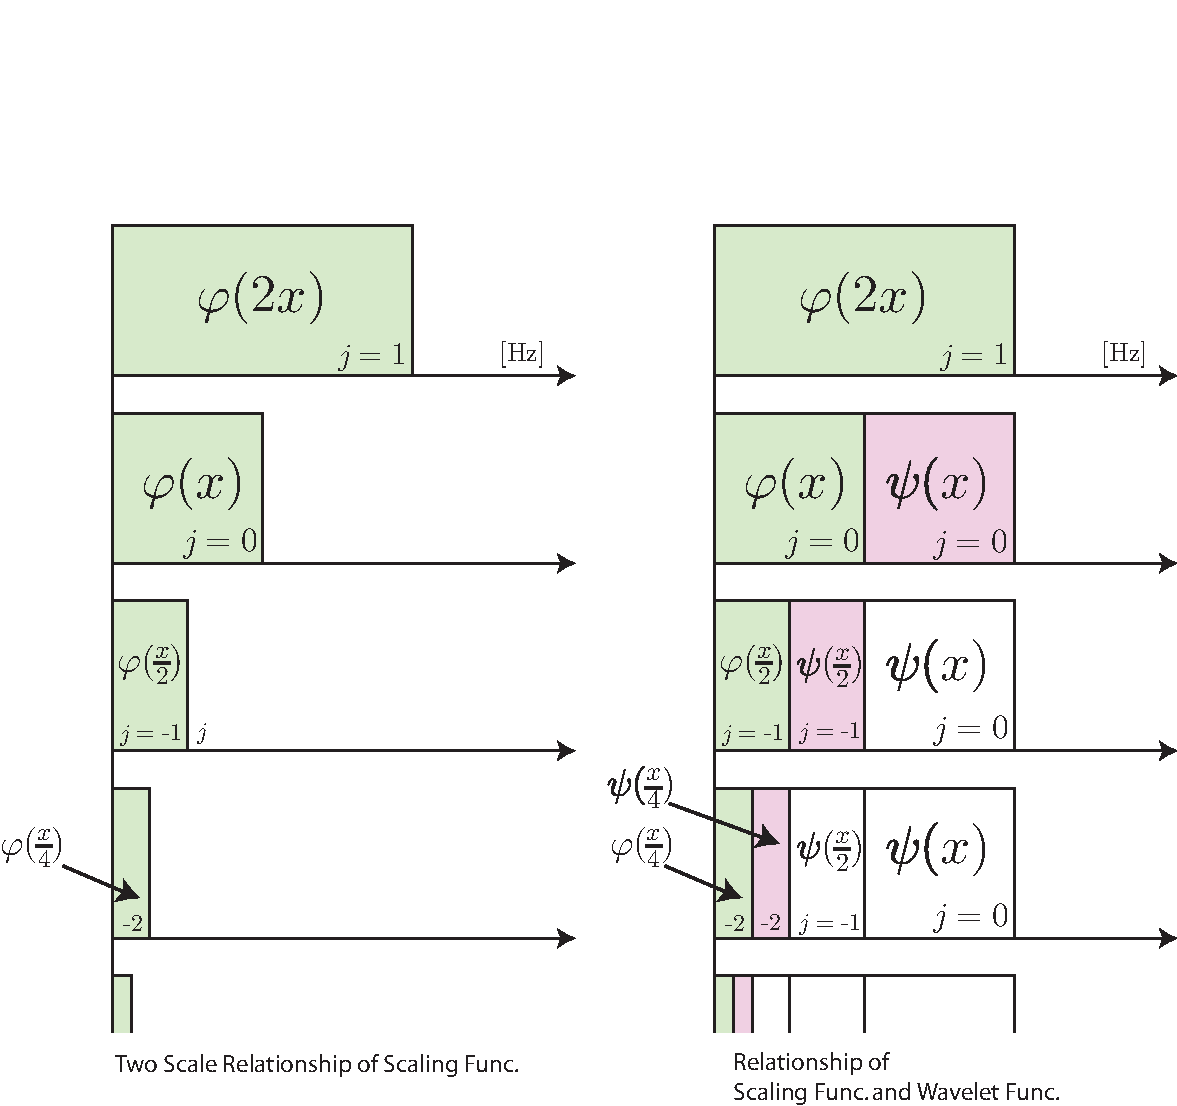
\includegraphics[width=3.5in]{chap1/fig/two-scale.pdf}
\caption{ツースケール関係} \label{fig-two-scale.pdf}
\end{center}
\end{figure}
算術符号は,区間を記号の出現確率に比例した小区間に分割して行くことで符号化を行う.
それでは例として,記号列abbbcを符号化してみる.式(\ref{eqAAAA})をみてね、。

\begin{equation}
S=\sum_{n=0}^N n^2 \label{eqAAAA}
\end{equation}
○○○○○○○○○○○○○○○○○○○○○○○○○ ○○○○○○○○○○○○○○○○○○○○○○○○○○○○○○○○○○○○○○○○○○○○○○○○○○○○○○○○ ○○○○○○○○○○○○○○○○○○○○○○○○○○○○○○○○○○○○○○○○○○○○○○○○○○○○○○ ○○○○○○○○○○○○○○○○○ ○○○○○○○○○○○○○○○○○○○○○○○○○○○○○○○○○○○○○○○○○○○○○○○○○○○○○○○○ ○○○○○○○○○○○○○○○○○○○○○○○○○○○○○○○○○○○○○○○○○○○○○○○○○○○○○○ ○○○
\section{だだだだ}
何か書く○○○○○○○○○○○○○○○○○○○○○○○○○ ○○○○○○○○○○○○○○○○○○○○○○○○○○○○○○○○○○○○○○○○○○○○○○○○○○○○○○○○ ○○○○○○○○○○○○○○○○○○○○○○○○○○○○○○○○○○○○○○○○○○○○○○○○○○○○○○ ○○○○○○○○○○○○○○○○○ ○○○○○○○○○○○○○○○○○○○○○○○○○○○○○○○○○○○○○○○○○○○○○○○○○○○○○○○○
\subsection{あああ} ○○○○○○○○○○○○○○○○○○○○○○○○○○○○○○○○○○○○○○○○○○○○○○○○○○○○○○ ○○○
\section{だああああ}
何か書く○○○○○○○○○○○○○○○○○○○○○○○○○ ○○○○○○○○○○○○○○○○○○○○○○○○○○○○○○○○○○○○○○○○○○○○○○○○○○○○○○○○ ○○○○○○○○○○○○○○○○○○○○○○○○○○○○○○○○○○○○○○○○○○○○○○○○○○○○○○ ○○○○○○○○○○○○○○○○○ ○○○○○○○○○○○○○○○○○○○○○○○○○○○○○○○○○○○○○○○○○○○○○○○○○○○○○○○○ ○○○○○○○○○○○○○○○○○○○○○○○○○○○○○○○○○○○○○○○○○○○○○○○○○○○○○○ ○○○


\subsection{基本的な考え方}
まず「算術符号」の{\gt 基本的な考え方について説明}する\cite{wavelet-2}.
算術符号は記号列,もしくは{\huge 文字列全体を\gt ひとつの符号語に}する方法であり,1960年代にP.Eliasによって提案された.\par
算術符号は,記号列を実数0と1の間の区間を用いて表す.たとえば,記号は{a,b,c}の3種類があり,
出現確率をそれぞれP(a) = 0.2,P(b) = 0.6,P(c) = 0.2とする.
算術符号は,区間を記号の出現確率に比例した小区間に分割して行くことで符号化を行う.
ここからは節\ref{QWERT}を参照してください。
それでは例として,記号列abbbcを符号化してみる.


\section{算術符号化}
sdssddsfsdds





\begin{figure}[htbp]
\begin{center}
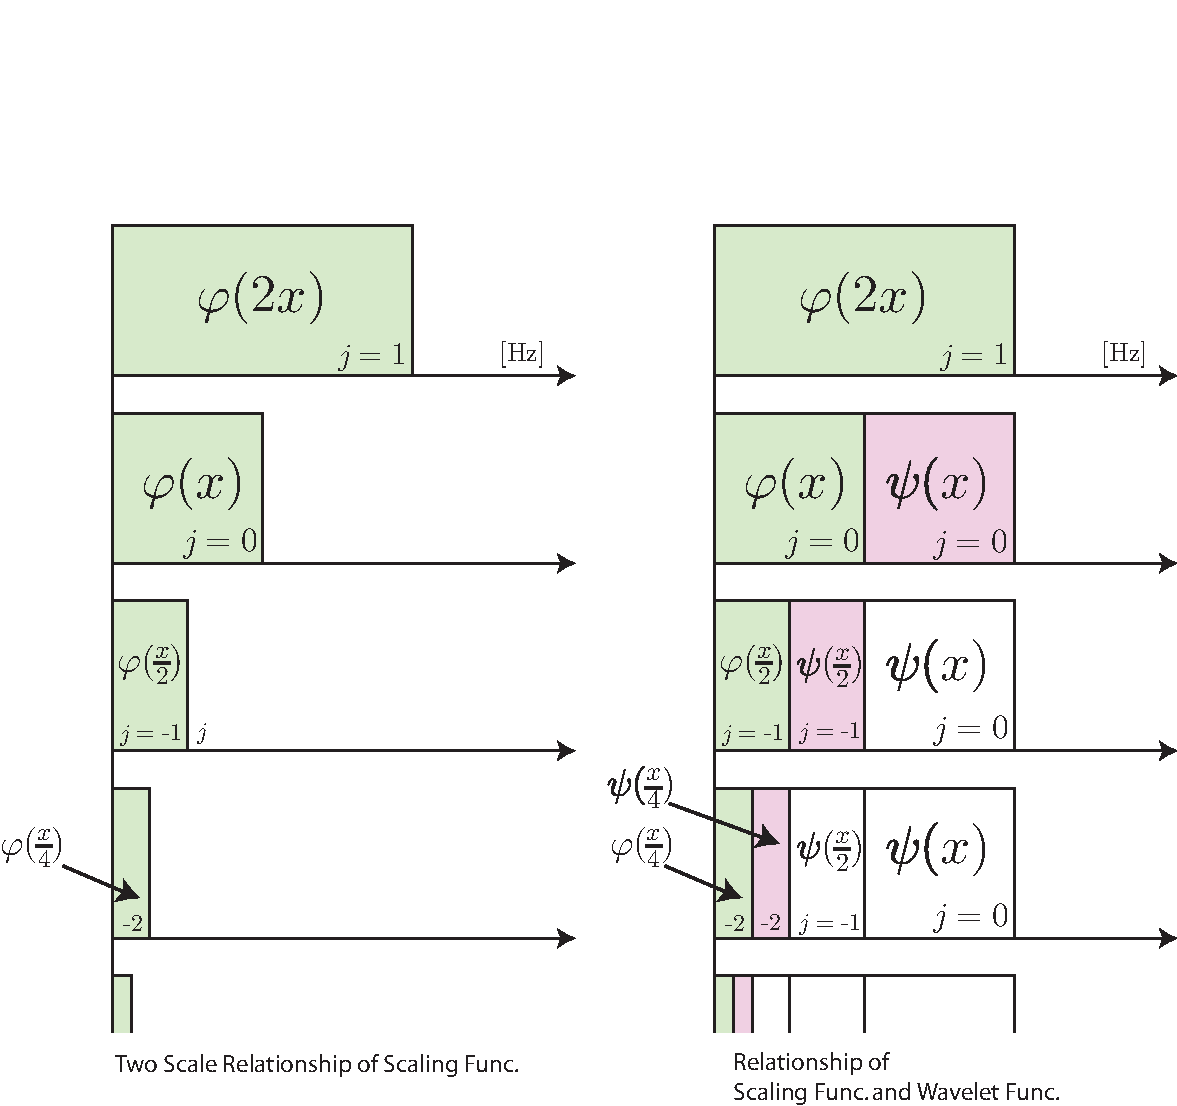
\includegraphics[width=3in]{chap1/fig/two-scale.pdf}
\caption{ツースケール関係aassad} \label{fig-two-scale.pdf}
\end{center}
\end{figure}

図\ref{fig-two-scale.pdf}に●●●を示す.


%% 大きなテーブルをいれるサンプル(longtable)
\begin{table}[h]
\begin{center}
\caption{言語別の特色}\label{AAB}
\begin{longtable}{|l|p{138mm}|}
\hline
言語 & 特色 \\
\hline
MySQL & あああああああああああああああああああああああ \\
\hline
Oracle & いいいいいいいいいいいいいいいいいい \\
\hline
SQL Server & ううううううううううううううううううう \\
 \hline
\end{longtable}
\end{center}
\end{table}



\subsection{平均符号長} \label{fugocho}
表\ref{tab:scores}に○○○を示す。リスト\ref{test.rb}に○○○を示す。


%%%%%%%%%%%% 図の挿入 %%%%%%%%%%%%%
\begin{figure}[htbp]
\centering
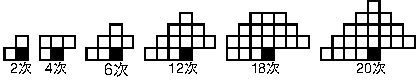
\includegraphics[width=\textwidth]{chap2/fig/tiger.pdf}
\caption{トラがでた}
\end{figure}

%%%%%%%%%%%% 数式
ベクトル$\bm{x}$とただの$x_0$
\begin{equation}
1+1 \C{うわあー!}
\end{equation}

%%%%%%%%%%%% 大きさをかえる
\scalebox{25.0}
{
あ
}
%
\begin{table}[htbp]
\caption{aaa}
\scalebox{5.0}
{
\begin{tabular}{cc}
あ & い \\ \hline
え  & お \\ \hline
\end{tabular}
}
\end{table}
